\documentclass{sigchi}

% Use this command to override the default ACM copyright statement (e.g. for preprints). 
% Consult the conference website for the camera-ready copyright statement.


%% EXAMPLE BEGIN -- HOW TO OVERRIDE THE DEFAULT COPYRIGHT STRIP -- (July 22, 2013 - Paul Baumann)
% \toappear{Permission to make digital or hard copies of all or part of this work for personal or classroom use is 	granted without fee provided that copies are not made or distributed for profit or commercial advantage and that copies bear this notice and the full citation on the first page. Copyrights for components of this work owned by others than ACM must be honored. Abstracting with credit is permitted. To copy otherwise, or republish, to post on servers or to redistribute to lists, requires prior specific permission and/or a fee. Request permissions from permissions@acm.org. \\
% {\emph{CHI'14}}, April 26--May 1, 2014, Toronto, Canada. \\
% Copyright \copyright~2014 ACM ISBN/14/04...\$15.00. \\
% DOI string from ACM form confirmation}
%% EXAMPLE END -- HOW TO OVERRIDE THE DEFAULT COPYRIGHT STRIP -- (July 22, 2013 - Paul Baumann)


% Arabic page numbers for submission. 
% Remove this line to eliminate page numbers for the camera ready copy
\pagenumbering{arabic}


% Load basic packages
\usepackage{balance}  % to better equalize the last page
\usepackage{graphics} % for EPS, load graphicx instead
\usepackage{times}    % comment if you want LaTeX's default font
\usepackage{url}      % llt: nicely formatted URLs


% llt: Define a global style for URLs, rather that the default one
\makeatletter
\def\url@leostyle{%
  \@ifundefined{selectfont}{\def\UrlFont{\sf}}{\def\UrlFont{\small\bf\ttfamily}}}
\makeatother
\urlstyle{leo}


% To make various LaTeX processors do the right thing with page size.
\def\pprw{8.5in}
\def\pprh{11in}
\special{papersize=\pprw,\pprh}
\setlength{\paperwidth}{\pprw}
\setlength{\paperheight}{\pprh}
\setlength{\pdfpagewidth}{\pprw}
\setlength{\pdfpageheight}{\pprh}

% Make sure hyperref comes last of your loaded packages, 
% to give it a fighting chance of not being over-written, 
% since its job is to redefine many LaTeX commands.
\usepackage[pdftex]{hyperref}
\hypersetup{
pdftitle={SIGCHI Conference Proceedings Format},
pdfauthor={LaTeX},
pdfkeywords={SIGCHI, proceedings, archival format},
bookmarksnumbered,
pdfstartview={FitH},
colorlinks,
citecolor=black,
filecolor=black,
linkcolor=black,
urlcolor=black,
breaklinks=true,
}

% create a shortcut to typeset table headings
\newcommand\tabhead[1]{\small\textbf{#1}}


% End of preamble. Here it comes the document.
\begin{document}

\title{DADS:Easier group collaborative affinity diagram through digital sticky-note creation and organization system.}

\numberofauthors{3}
\author{
  \alignauthor William Widjaja\\
    \affaddr{Department of Management of Science and technology Human interface lab, Tohoku University}\\
    \affaddr{Aobayama 6-6-01-2, Sendai, Japan}\\
    \email{william.widjaja
    @most.tohoku.ac.jp}\\
  \alignauthor Haruna Hayasaka \\
    \affaddr{Department of Quantum-Science Lab, Tohoku University}\\
    \affaddr{Aobayama 6-6-01-2, Sendai, Japan}\\
    \email{haruna.hayasaka
    @luke.qse.tohoku.ac.jp}\\   
  \alignauthor Masayuki Sawamura \\
    \affaddr{Department of Quantum-Science Lab, Tohoku University}\\
    \affaddr{Aobayama 6-6-01-2, Sendai, Japan}\\
    \email{masayuki.sawamura
    @luke.qse.tohoku.ac.jp}\\
}

\maketitle

\begin{abstract}
Problem solving in groups or teams requires individuals to exchange and organize their opinions in order to reach a solution. A popular method for structuring these idea exchanges is the affinity diagram. Creating an affinity diagram involves each member of a team writing individual opinions on sticky notes and making groups and links between these opinions with others by moving and arranging the sticky notes on a common wall or whiteboard. Despite being a standard business practice, this traditional paper-based method can be improved by integrating new technology. The Digital Affinity Diagram system (DADS), a digital sticky note creation and organization system, integrates private creation and common organization spaces in one computer environment. Using an extended dual-monitor setup to separate the two spaces, individuals can build stronger personal opinions by attaching references in a private space, and collaboratively organize group opinions in a cross-terminal synchronized common interactive space.  We present a comparative study to determine which of the two methods is more usable for group practice. 
\end{abstract}

\keywords{
	CSCW;Collaboration; Affinity-Diagram; Brainstorming; Group work; Sticky-note 
}


\category{H.5.1.}{Information Interfaces and Presentation (e.g. HCI)}{Miscellaneous}

\section{Introduction}
Exchanging and organizing ideas between groups is an integral part of group problem solving. One such method commonly used to exchange and organize ideas between people is called Affinity Diagramming\cite{kawakita1991original}. Affinity Diagrams are often created by writing individual ideas on sticky notes and, together with other participants, move and arrange the notes to create groups and links in accordance with the ideas' similarities. While brainstorming is widely used as a method of idea generation, there is less work on how groups can deepen ideas, or how they can use structural changes to increase understanding.\cite{dickey2012framespaces} E-collaboration presents many opportunities to change traditional analog methods for the better in these respects.

In this paper, we introduce the Digital Affinity Diagram system (DADS), an e-collaboration tool that implements an individually-controlled multi-user synchronized affinity diagramming system. DADS allows each user to control digital sticky notes while concurrently synchronizing the visual movements across multiple users' screens in real-time. Synchronization is achieved by using a low-latency, highly optimized network socket server which updates and broadcasts each manipulation command at a high frequency. This technology allows multiple users to collaborate in creating affinity diagram together in a single sandbox. To show the system's usefulness, the current experiment compares it to a traditional method of affinity diagram creation using sticky notes. 

Our system is inspired by similar work in virtual workspaces and e-collaboration tools, but differs from them in important ways. DADS separates common from private space in the idea creation phase so that users can compose and support their idea before putting it in public view. Separating common interactive space and private interaction space helps to alleviate users' anxiety, making it uniquely suited to discussing sensitive topics, or by cross-departmental teams who may not share the same level of expertise on all topics. Managing face threat and encouraging production are important problems in the study of group creativity. Separating common interactive and private input spaces has been proposed as a solution to brainstorming processes that are slow to start due to participants' anxiety\cite{paulus2000idea}. Digital systems provide a "screen" for introverted or uncertain users, and the explicit creation of a private space reduces production blocking in the brainstorming process \cite{brown1996simple}. In the system we present, users have the space to build confidence in their ideas before being subjected to critique by their peers.

Our system further improves upon this process, using technology to circumvent some of the challenges of group dialogue, and at the same time providing users with new capabilities when conducting idea-exchanging activities. By leveraging commonly available and familiar technology, we have designed a user-friendly collaborative system to support and augment the affinity diagram process. We have incorporated three major functions that make e-collaboration on affinity diagrams using DADS easier than analog collaboration: the attachment system, the comment system, and an intuitive interface that simplifies navigation between ideas. The attachment system allows collaborators to attach text, images, and media to their ideas to give them context. We believe this system will allow users to better understand one another in discussions. Similarly, e-collaboration will make commenting and understanding others' comments on ideas easier, leading to more productive refinement of ideas and higher quality discussion. Finally, the 3-column interface for creating, annotating, and browsing others' ideas makes navigation smooth and allows users to focus on content.

We operationalize usability in three ways: a usability survey administered to participants, a more general System Usability Score, and several behavioral performance metrics. Our analyses determine which of the two methods is more preferred by users and whether DADS supports users in exchanging and organizing their ideas.

\section{Problem Space}
There are problems with exchanging ideas face-to-face. Original KJ/brainstorm method promotes shallow ideas by not providing enough room on sticky notes. Other e-collaboration tools do not solve this problem. 

\section{Previous Research}
Other attempts to solve this problem have focused on exactly replicating the physical constraints in a digital format, as in Geyer and colleagues' Affinity Table\cite{Geyer:2011:DRI:2069618.2069647}. Their device allows users to create virtual sticky notes with digital ink and move them around via a multi-touch surface. Similarly, Miura and colleagues' Group KJ system used digital pens to encourage as much similarity between the digital and analog process as possible, and focused on the record-keeping advantages of a digital system\cite{miura2011gkj}. Both of these systems retain some of the problems of the physical process of creating an affinity diagram: namely, negotiating physical space with others (the "seating arrangement" problem\cite{patterson1979effects}), and the space allowed for idea expression. While larger groups have been shown to produce more creative and higher quality ideas during brainstorming\cite{gallupe1994blocking}, affinity diagrams are usually limited to a smaller group due to space limitations. Our system takes a different approach, augmenting the affinity diagram process with tools that can increase the level of detail included in an idea without increasing the visual real estate required. Studies of digital proxemics\cite{ballendat2010proxemic} suggest that mediated interactions should encourage and supplement existing human interactions and goals. In the case of affinity diagrams, current digital implementations fall prey to the same errors in proxemics that the analog version does - individuals compete for space and public-board real estate instead of focusing on creating persuasive and relevant ideas. By giving each participant their own access to the public board through a multi-touch auxiliary monitor, our system eliminates this competition for space. Using DADS, every participant has equal access to the public idea space at all times. 

We also incorporate color-coding of notes to identify authors, which reduces the anonymity of the digital process. Instead of a system that promotes neutrality, like that developed by Tse and colleagues\cite{Tse:2008:ETM:1394445.1394457}, we developed a system that promotes investment in ideas and  encourages authors to strengthen their argument for a particular opinion or solution. We do draw some features from Tse's earlier model, namely grouping and linking movements that can be executed in the public arena. In addition, his notion that personal and group territories should be overlapping is reflected in our system by the access each participant has in their private input space to a list of all other points that users have made on the topic. This feature also incorporates a function inspired by a thesis by Jonas Minke\cite{publication-4659} that highlights the difficulty of searching for particular sticky notes in an affinity diagram. One solution using a digital affinity diagramming system would be to make notes searchable in a list format, which is much more visually tractable. We discuss this feature further in our explanation of the private input space in the DADS interface.


We are also inspired by another line of research on idea creation and organization that comes from collaborative web-browsing tools. Paul and Morris' CoSense tool enables group web-based investigation by making better sense of how individuals reach solutions and look for information to support them.\cite{Paul:2009:CES:1518701.1518974} In our experiences with affinity diagramming, we often found that a sticky note was much too small for some of the ideas that users wanted to contribute, especially if the process required people to express persuasive opinions. Therefore, we developed an augmented affinity diagram system that draws from both digital implementations of the affinity diagram process and from collaborative investigation tools like CoSense.


\section{System Architecture}
The research we have reviewed above gives us four areas to focus on, where our digital system could improve upon previous work. These four areas are: creation, presentation, the exchange of opinions, and the creation of a collaborative affinity diagram.


\subsection{Creation} The most important feature of a digital collaboration system is to give users the ability to quickly and simply create representations for their ideas that can be shared with other users. The ability to create and share ideas is heavily influenced by users' ability to navigate the system, especially any input mechanisms. Our system provides an intuitive 3-column interface that enables users to create new items and populate them with content, and easily switch back and forth between viewing their own and others' ideas. The idea viewing section is divided into two areas (Title and Contents) which we believe will help users formulate their ideas more clearly. The attachment feature of the system is also crucial here: since supporting one's ideas frequently involves looking something up on the Internet, even in everyday conversation, we needed to provide an intuitive link between the idea creation area and sources of online information. One of the simplest functions is the cut-and-paste mechanism that can allow users to directly quote a website source. Users can also select images to include in the support for their idea. We also allow users to capture a screen shot of any website if they wish to quickly include text and images, or the image is not in a standard format. URLs and images are quickly processed into a thumbnail format that can be expanded by the user or viewer.
\subsection{Presentation} One major focus of this project is helping users express themselves better during group discussions. To this end, we decided to synchronize the opening and closing of cards using the expansion system so that it can be used as an explanation tool. During the Presentation phase of the experiment, users can expand images that they attached to their idea card to further support their claims and ideas. Card and image expansions are synchronized across all users' common interactive boards and the central common view screen. The opening of images, URLs, and PDFs, zoom-in and zoom-out functions, and scrolling navigation are synchronized across all users so that the documents supporting presentation are part of a seamless shared experience. In addition, since users in the U-shaped seating arrangement may not be able to see the presenting user's hand, we built a special digital pointer tool that lets users highlight areas of the screen or indicate a certain passage of text. The digital pointer is incorporated across all image and page handling systems within the digital environment, including the internal browser.
\subsection{Exchanging Opinions} An important function of group discussions is to exchange opinions, critique ideas and think of improvements. While the easiest way to refine ideas in a group is probably through conversation, recording and accurately interpreting conversations is problematic. Using a text-based comment system is a better choice for groups that need to keep an accurate log of discussions, refinements, and next steps. Also, text-based comments allow users to simultaneously add their opinions to the discussion without interrupting anyone else, reducing the impact of production blocking and social coordination. 
In our system, users can write a comment on any point, which logs their comment and attaches it to that point. This keeps the comment system on-topic and prevents it from getting confused. We also incorporated a notification system so that users can keep track of comments that are left on their ideas. This is represented as a small dot that shows up on the idea creator's screen when someone leaves a comment. Users can cancel this notification by scrolling to the bottom of the list of comments briefly, at which point the system logs the comment as "read" and cancels the notification dot until a new comment arrives.

\subsection{Collaborative Affinity Diagram}

\subsection{Hardware Setup}

We designed a three-person seating arrangement with synchronous access for this experiment. The system can further accommodate 4 or more individuals, and allows an asynchronous option when remote access is required. The current setup demonstrates what we imagine will be the most common use of the system, to facilitate face-to-face Affinity Diagram creation meetings for small teams. 

\begin{itemize}

\item \textbf{U-shaped Seating Arrangement} - This seating design optimizes the dual monitor system and proximity between each participants. In our 3-person experiments, a large monitor acts as a shared common screen visible by all participants. Even though all secondary screens are synchronized, the large screen serves to assure participants that their manipulations and additions were recorded and synchronized with all other users' boards. 
\item \textbf{Extended Dual Multi-Touch Monitor} - For each user, their main laptop is located centrally, while their external monitor is to their left side, giving space for the mouse on the right side. We chose to use a multi-touch enabled monitor tilted at 30 degrees, to give users best access to the common interactive space as a virtual 'drawing board,' and also allow eye-level contact for increased gaze awareness between users. 
\item \textbf{Server Setup} - Our server uses Windows 8, which acts as a database system and a synchronized input-output traffic center. The server does not require high performance for less than 5 simultaneous participants, and rather than high speed performance, the system prefers low latency in order to allow the high-frequency refresh of simultaneous workspaces.
\end{itemize}

\subsection{Software design}

DADS was designed and developed at Tohoku University's  utilizing the latest agile methods in software development engineering and strict usability testing methodology to achieve a consistent development pace. The team focuses only on using technology that is easily available on the market and leverages highly designed software development capabilities to create a high-quality product with superior user experience for supporting group discussion. The basics of the system can be seen in our previous work, the Discusys system\cite{widjaja2013discusys}. The current system presents several technical and design improvements.


The system's software was developed using C\#, mainly Microsoft's .Net 4.5  framework. We built the software natively, choosing Microsoft libraries over other .Net open-source libraries to increase compatibility across critical server, database, and client infrastructure. In addition, we also took advantage of the touch framework library that is currently maturing in Windows 7/8. This library allowed us to include a large screen multitouch monitor in our solution. We utilize a traditional laptop system running Windows 7 and extend the screen with a 22" Iiyama multitouch monitor. The multitouch monitor uses a four-point infrared sensor to detect accurate multitouch from users, and has an 8ms response time. We chose a dual-screen design to increase information display clarity and focus for the users. While the main Private input screen will act as each user's personal input interface,  the common interactive space  will focus on collaboration. 

\subsubsection{Real-time Synchronization Technology}

To synchronize events and operations between severs and multiple clients, DADS relies on a network
socket infrastructure called Photon Engine, created by Exit Games. It is designed for use in MMOGs, and provides reliable low-latency data transport services on top of a user datagram protocol (UDP). Photon can also be used as a Remote Procedure Call (RPC) system and server-side runtime for Application logic. Photon Engine acts as a delivery medium for code execution and callback between multiple clients and servers. For example, if the client calls some code on the server side, the server-side code executes and may return some arguments back to the client. The benefit of Photon is that it serializes the code logic by packeting it in small bytes of integers and creating a continuous call for event updates (up to 10 update calls per second) to simulate synchronous real-time behavior. Without Photon, we would have to deal with network packets directly, either using TCP/IP or UDP sockets. This would lead to an inefficient code execution stream, and increase latency in the system. Photon handles all instant notification needs, including: 1) All updates created by users, 2) All operations on the common interactive space editor (interactive user cursors, moving and editing any shapes), 3) Logging statistics of operations for further analysis. In sum, the Photon Engine server application will process all of DADS' main functions and automatically update any changes made to the SQL server database in real-time.


\subsubsection{Private Input Interface}

The private input interface is designed to maximize visibility and navigation capabilities for users viewing both their own points and others' points. Following network socket design standards, each discussion topic is treated as a separate room. Users are asked to give their name and select a color to represent their points on the common board. After identifying themselves, they choose a discussion room to participate in, and upon entering, each user can be identified by their chosen color. Giving each participant an identifying color parallels the practice of giving participants a unique color of sticky notes with which to perform the Analog affinity diagram task. This links ideas to their author and increases the personal dimension of interaction that can sometimes be lost in digital methods\cite{ballendat2010proxemic}.  

There are 5 separate areas in the private dashboard. The private input interface is a workspace intended for users to create points by inputting ideas and information. Figure 1 shows the 3 column dashboard: in the top right hand users can select different topics and switch from one topic to another; the middle column lists all the opinion titles written by each participant; the bottom right corner is where users select and view different participants' points; the lower center column lists the titles of other participants' points. Finally, the full screen right-hand column is where users construct their own points. Three distinct areas allow users to give each idea a title, description, and source documents that support each idea. 

\begin{figure}
\centering
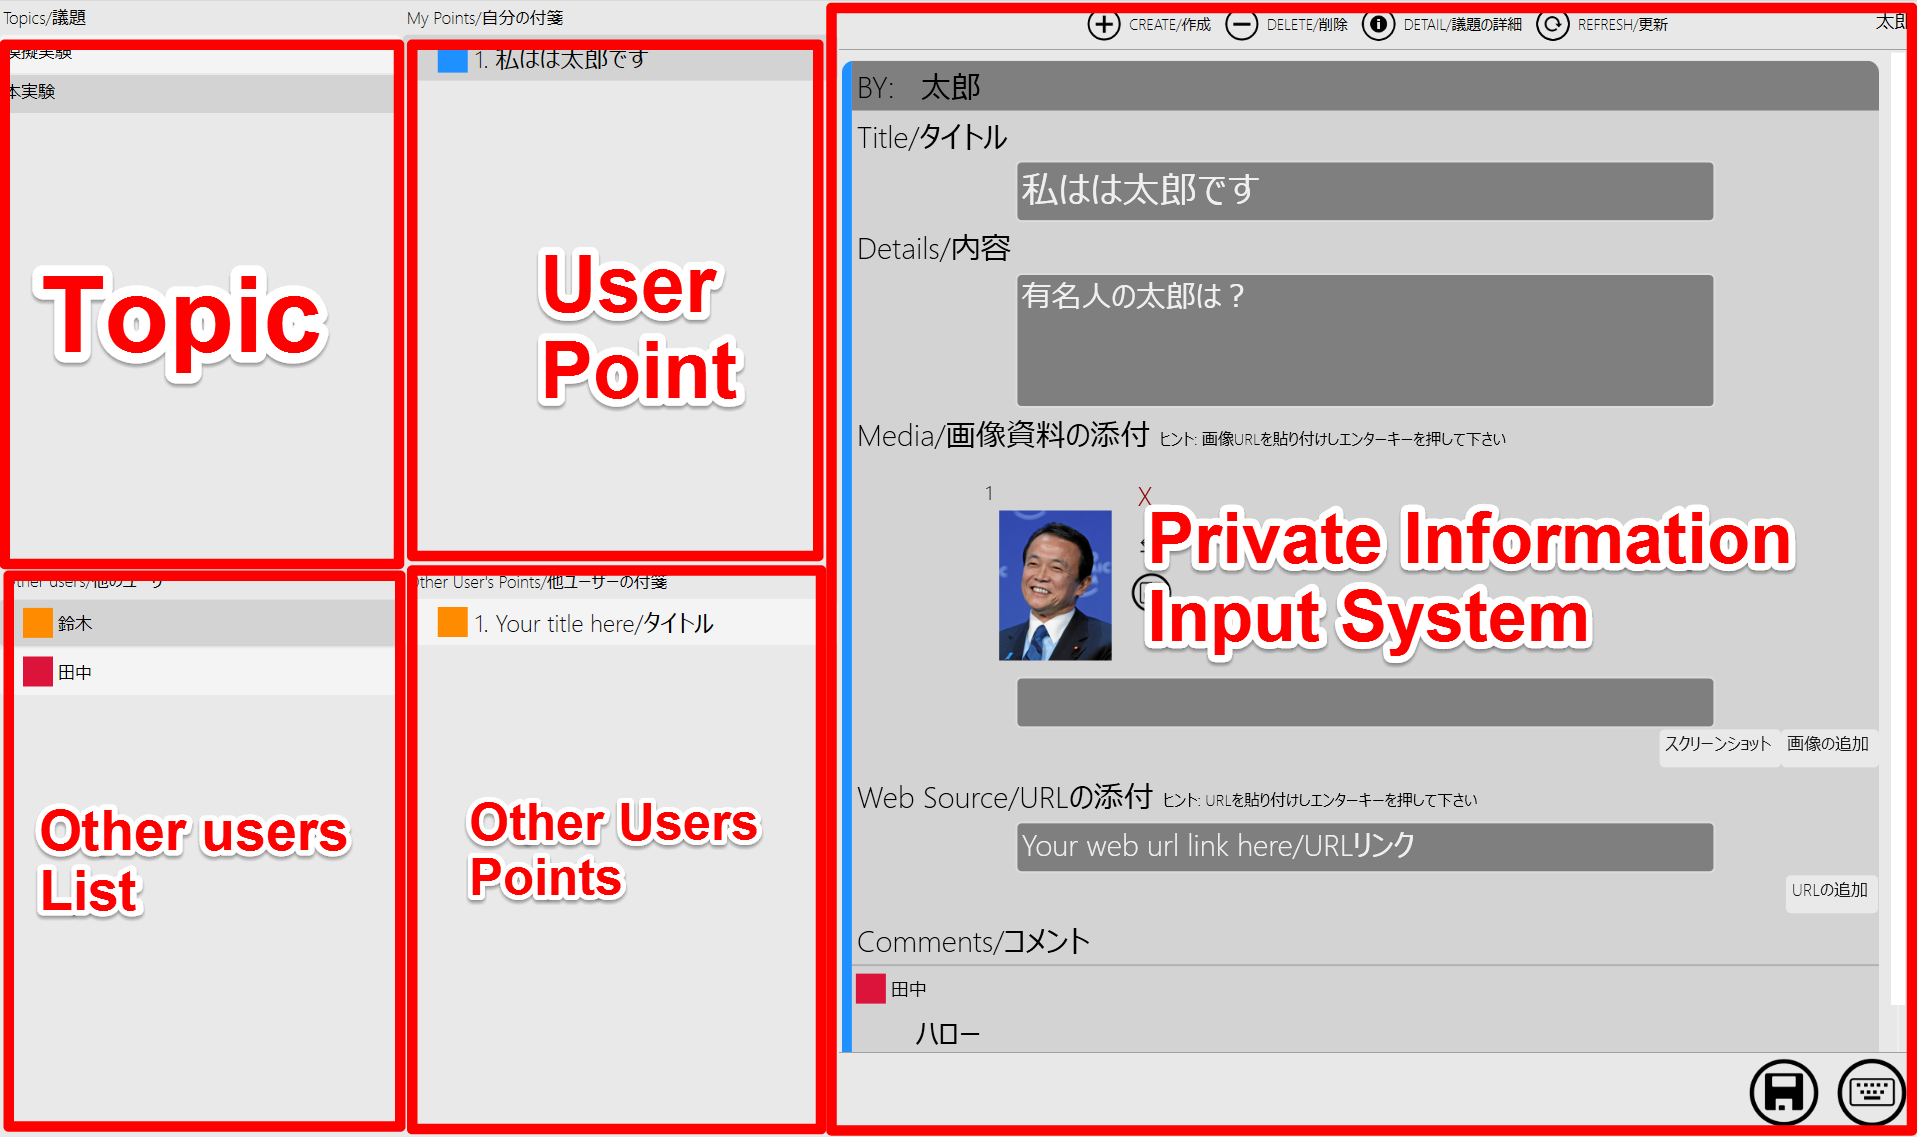
\includegraphics[width=1.0\columnwidth]{private}
\caption{Private Space User Interface}
\label{fig:figure1}
\end{figure}

Users can switch freely between the input dashboard and a browser window when they are searching for supporting material.  Early in the development phase, we observed that users often search for more information on the Internet to verify or affirm their ideas. To support this behavior, our system's source attachment function gives users the ability to attach articles or sources from the Internet to their ideas. We included three features that allow users to enhance their ideas with evidence: Internal Browser, Media Attachment, and Screen Shot. The system's internal browser makes it easier for participants to search of evidence to support their ideas. In addition, they can include URLs in their supporting material which will open naturally for other users. Media Attachment allows users to employ the familiar copy and paste functions to upload images from the web. While using the Internet browser, users are able to right-click the images they wish to upload and copy and paste the image url to our media text box in the system's private input form. The system automatically detects the presence and format of media, prompting users to correct badly formatted URLs and showing thumbnails of successfully processed images. We also observed that some users wanted to capture whole areas of a website, or graphics that are not in a standard image format, so we also incorporated a screenshot function. After pressing the screen shot button in our system, the internal web browser will be displayed, and users can scroll up and down to the desired part of the page. Clicking on the screen will initiate the capture window, and letting go of the drag window will capture the screen selection. The screen shot thumbnail is automatically displayed in the private input screen, indicating that the capture was successful. 

The private space interface allows users to easily create points related to a topic and populate them with information using familiar cut-and-paste mechanics. A basic interaction process would involve selecting the topic from the Topic window (pictured in Figure 1) and creating a new point in the User Point window, which creates a new card on the common interactive  space related to that topic. Users can be identified as the author of a point by the color of the card. Users can also view all of the other points made in two locations: the common interactive board, and the bottom of the center column. This immediate availability may increase creativity by discouraging repetition and allowing implicit collaboration even before the collaborative affinity diagramming activity has begun. After creating a point, users can illustrate their point by adding supplementary information, images, and links in the Private Information Input window. Users can also use the built-in Internet browser in order to get more information or media to illustrate their point. When they are done adding information, the card is complete and they can create a new point, or browse other users' points, just as in the analog version of AD creation.


\subsubsection{Common Interactive Space}

\begin{figure}[!h]
\centering
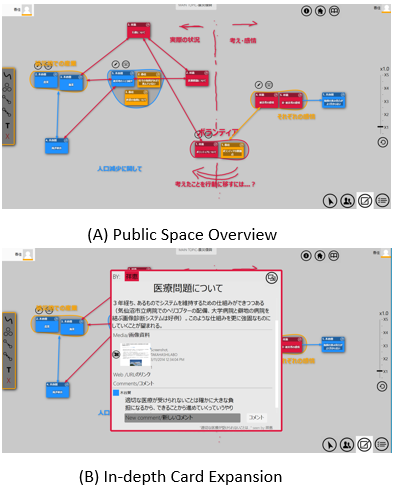
\includegraphics[width=1.0\columnwidth]{public4}
\caption{(A) Screenshot of common interactive Space interface with groups and links (B) Card Expansion: double tap gesture expands the selected card to display in-depth information including details, images and comments}
\label{fig:figure1}
\end{figure}
In the common interactive space interface, points written in the private input space are displayed as cards with the author's identity color. The card also displays the point's title and the author's name. These cards can be rearranged by touching and dragging them to a new location on the multi-touch screen.

We believe that successful collaboration requires the common interactive  space to be synchronized smoothly across different users. To achieve this goal, we utilized the Photon Engine, core technology from a MMOG system that uses network sockets, and adapted the technology to suit our system. Participants are treated like players in a MMOG system, with a unique identity and the ability to manipulate idea boxes and enlarge the details of other participants' ideas. These manipulation input commands are constantly sent to the server, and updates are broadcast to other clients at up to 10 commands per second.  Low latency will determine the smoothness of the common interactive  space's control and manipulation responses. 


Five key features of the common interactive space allow users to assemble an affinity diagram as easily - or more easily - than they can with the traditional sticky-notes-and-pen "analog" method.

\begin{itemize}


\item  \textbf{In-depth Card Details} - Cards on the common interactive display only the title of the user's idea. Users can expand the card details by double-clicking on the card. This triggers a window that displays all of the in-depth information that the author included in the idea's supporting materials, including the description, attached links, and media sources. 
\item  \textbf{Presentation Mode} - Card expansion actions are individually controlled by default. Users can also synchronize card expansions between users or across the whole teaming order to help users control and present their ideas easily, especially during the explanation phase of Affinity Diagram creation.
\item \textbf{Grouping and Linking} -  Grouping and linking cards can be accomplished using certain motions on the multitouch monitor. If a user presses the 'Group' button and touches cards on the common interactive space with a circular motion between several cards, a border around these cards is created, and these grouped cards can be moved as a unit. Groups of cards can be reorganized by moving any card within the group. Inserting new cards into an existing group happens if any 2 corners of an ungrouped card touches the group. If this occurs, it initiates a regroup function that allows users to insert a new card into the group. Users can link cards or groups to each other by pressing the 'Link' button and clicking two cards in sequence.  
\item \textbf{Vector Free Draw Annotation} - This feature allows users to draw a free-form vector object in the common interactive space that can be moved and re-sized. Editing these objects can be done with a stroke-by-stroke undo process instead of the cumbersome and graphically unappealing eraser function. Unlike the group boundaries and link lines, these objects allow users more flexibility to create symbols and diagrams on the spot, following the design principle that "a picture is worth a thousand words."  
\item \textbf{Commenting System} - This function replicates the commenting phase of the analog Affinity Diagram process by allowing users to comment on each other's ideas, ask questions, and write comments via the system. Users can expand any card and write comments on another person's ideas. In addition, users are notified of new comments via the system, which allows users to have real-time exchanges with each other. 

\end{itemize}



\subsection{Methods}

This experiment compares the analog method of affinity diagramming to a new digital approach using the system described above. The affinity diagram process was originally developed to overcome some of the problems inherent in brainstorming and exchanging ideas\cite{kawakita1991original}. The Nominal Group Technique (NGT) refines the process used in creating affinity diagrams. This technique is particularly helpful for groups that have not worked together before, are imbalanced in terms of extroversion/introversion, when the topic is controversial, and when some quantitative output is desired. Groups using NGT reported that this technique increased feelings of accomplishment and group efficiency compared to freely interacting groups\cite{gallagher1993nominal}. 

During the creation of a collaborative affinity diagram, users go through 5 phases in the NGT:  
\begin{enumerate}
\item Introduction and explanation
\item Silent generation of ideas
\item Sharing ideas by posting them on an open white board
\item Group discussion
\item Voting and ranking
\end{enumerate}
This process was developed for problem-solving situations where groups had to agree on actionable next steps \cite{delbecq1971group}. Our process focused more on generating ideas and making associations between them rather than arriving at the best solution for a specific problem. Therefore, we eliminated the Voting and Ranking phase and ended our process after the creation of idea groups by users. 

Discussion topics for this experiment were designed to provoke many ideas and perhaps even heated discussion that would be moderated both by the NGT structure and by the use of digital tools. Both natural disaster recovery and nuclear energy have become important topics in Japan since the 2011 Tohoku earthquake. Naturally, most people in Japan have an opinion about how these crises have unfolded, so we thought these would be productive topics for discussion. We asked participants to discuss one of two topics in each experiment condition:

A) Nuclear Energy
B) Disaster Recovery 

In order to test the usability of our system against traditional methods, we set up two different idea exchange environments which we refer to as Analog and Digital methods. In the analog method, traditional tools are used including a whiteboard, colored sticky notes, and colored markers. Ideas and comments are written on numbered sticky notes. Users write their idea's title using a marker, and comments are written using a black pen. Comments are pasted below the relevant idea note, creating a physical connection between the ideas and comments. To make the experiment equally balanced, we allowed users in the Analog condition to search the Internet and print out any sources they wished to use. Magnets were provided to help connect these printed materials to the idea notes. In the Digital environment, users interacted with our system to conduct the experimental tasks. Before the experiment, participants were given instructions and a tutorial on how to use the system. Upon completing the experiment, participants were invited to participate in a survey comparing and evaluating the system's usability on a number of dimensions.

\subsection{Procedure}

Materials and experiment instructions were in Japanese, the native language of all participants. Because of our sample's homogeneity, we could rely on participants' cultural identity to drive some interest in the controversial discussion topics we chose.

In this experiment, we compared the Analog and Digital methods of Affinity Diagramming within groups of 3 individuals. Having an odd number of participants per group prevents sub-groups from forming - for example, 2 groups of 2. Users were given a different topic for each affinity diagram; they either discussed the recent earthquake recovery process in Japan, or recent developments in Japan's nuclear energy policy. Each group created one Affinity Diagram using the analog method and one in the digital method. These topics and the order of conditions was counterbalanced across groups, so that an equal number of teams had the Digital condition + Earthquake topic first, an equal number had the Analog condition + Nuclear topic first, and so forth. Each diagram went through 4 phases of creation, listed below.

Participants were welcomed and introduced to the purpose of the study and given a 20-minute overview of the tasks involved. If the group was assigned to the Analog condition first, they were given 30 minutes of instruction on how to create a collaborative affinity diagram using sticky notes, markers, and a white board. If they were assigned to the Digital condition first, they were given a 60-minute tutorial on using the digital system to create, support, present, comment on, navigate between, group, and link ideas in the creation of a collaborative affinity diagram. Participants had ample time during this tutorial to try out the system in the tutorial mock-up scenario, to become familiar with the system, and discover system functionality. The digital condition required a longer tutorial time in order to ensure that users were reasonably comfortable with the system. Users confirmed their familiarity with the system's functions in a quiz at the end of the tutorial. Groups completed all four phases of one condition using one discussion topic before switching to the other condition and using the other discussion topic.

\begin{itemize}
\item \textbf{Task 1: Idea Generation and Attach Source} - Users create new ideas based on his or her opinions and perceptions of a single topic. During the idea creation phase for both Analog and Digital conditions, users can employ internet searches in two different typical behaviors. One is to start writing immediately, and use internet-based information to verify their ideas. The other behavior is to search for inspiration on the internet first, and write down ideas based on information discovered in their search. Both idea creation patterns benefit from attaching internet sources (images or URLs) to their ideas. Each user was given 30 minutes to create 5 ideas on the assigned topic. They are given access to the Internet to search for support for their ideas. 
\item \textbf{Task 2: Present ideas to others } - Even though ideas are always visible on the common interactive space board, having ideas explained by their creator is more persuasive than merely reading them. Therefore, our goal was to build a system that helps users explain their ideas easily. We believe that the availability of sources to support ideas will increase users' confidence. A system that allows users to control and broadcast their sources during the explanation phase will increase ease of explanation for idea creators, and increase the whole team's level of understanding. Each user was given time to present and explain their ideas to the other participants; this stage took about 15 minutes. 
\item \textbf{Task 3: Exchanging comments } - Each idea is unique, and in order to understand them team members must be free to question and critique. Thus, easy navigation to specific ideas must be a priority in the commenting system. The exchange of ideas is facilitated by the same turn-taking mechanisms that operate during conversation. Therefore, our system notifies users when a new comment has arrived, and users are able to reply immediately. The group was given 20 minutes to comment on others' ideas and reply to any comment posted to them. They were asked to write as many comments as possible across all the ideas, until the time was up. 
\item \textbf{Task 4: Affinity Diagram creation} - The Affinity Diagram process is a common feature of Six Sigma organizations. It is used in business and academic settings to help a group organize their ideas around a specific topic. This simple method groups and links similar and related ideas in order to increase clarity and simplicity. This exercise is a precursor for any problem solving task, and can help teams create more effective solutions based on a unified view of the problem space.  After commenting on each other's ideas, participants were asked to collaborate on an affinity diagram using the ideas created earlier, grouping similar ideas and linking related ideas using a Nominal Groups technique which was explained to them in the instruction phase. This stage took about 15 minutes.
\end{itemize}

After completing the task in one mode (Digital or Analog), groups were given a long break before returning to complete the experiment. All participants completed all 4 tasks in both analog and digital methods, for a total of 8 tasks in each experiment group. The total time needed to complete both conditions of the experiment (with breaks) was 5.5 hours per group, on average. To show the equivalence of the two methods, a snapshot of each experimental condition is shown in Figure 4.

\begin{figure}[!h]
\centering
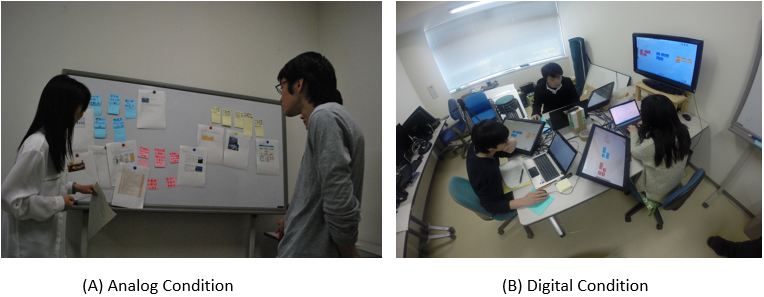
\includegraphics[width=1.0\columnwidth]{condition}
\caption{(A) Analog Condition: using sticky note and white board (B) Digital Condition using DADS with auxiliary multi-touch monitors.}
\label{fig:figure1}
\end{figure}

\subsection{Instruments and Measures}

This experiment presents us with the opportunity to measure both performance on the tasks involved in creating affinity diagrams, and participants' experience of performing these tasks. We created a detailed survey about specific features and affordances of the digital and analog conditions, and we also used the Standard Usability Survey to measure the digital system's usability and learnability. We use a linear regression method to shed light on interesting relationships between the survey responses, SUS scores, and performance metrics.

\subsubsection{Survey and Performance Analyses}

We designed a post-experimental questionnaire with 15 1-5 Likert scale rating questions addressing how easy or hard it was to perform certain tasks using either the Digital or the Analog method. For the questionnaire, low scores indicate less reported usability. Questions are listed below with a short ``nickname'' so that our results can be more easily understood. Our specific questions were:

\begin{enumerate}
  \item How easy was it to create ideas using this system? (Create)
  \item How easy was it to edit ideas using this system? (Edit)
  \item How easy was it to attach sources to your ideas using this system? (Attach)
  \item How easy was it to explain resources and support for your points in this system? (Show)
  \item How easy is it to explain your points to others? (Explain)
  \item How easy was it to read other users points in this system? (Navigate)
  \item How much do you understand other person points? (Understand)
  \item How easy was it to read comments on others' ideas in this system? (Read)
  \item How easy was it to write comments on others' ideas in this system? (Write)
  \item How easy was it to reply to comments in this system? (Reply)
  \item How easy was it to create an Affinity Diagram in this system? (Flexible)
  \item Which of the two environment is easier  you to cooperate with other group members to achieve the task?(Teamwork)
  \item How comfortable do you feel during the experiment?(Comfort)
  \item How useful do you think this method is compared to the other method you experienced? (Useful)
  \item How satisfied are you with the final Affinity Diagram that you made using this method? (Satisfaction)
\end{enumerate}

We measured several aspects of individual users' behavior in order to get a clearer picture of what users did in each of the conditions: number of attachments made, number of comments made, number of times a card was moved, grouped, or linked, and the amount of time groups took to create the final affinity diagram. We also calculated the number of moves per minute for each user; we view this measure as an indicator of the cognitive agility afforded by each system. Groups' behavior was recorded automatically in the digital environment. In the analog condition we used a GoPro HERO3+ digital video camera mounted on a jib in order to provide visual access to all users' movements. Video from the analog condition was hand coded by the first author.

\subsubsection{System Usability Scale}

The SUS provides an efficient way for users to evaluate a new system based on its usability and learnability. It measures the effectiveness, efficiency, and satisfaction of any new system and can be adapted to assess hardware, software, and business processes. The SUS has 10 questions, making it easy for participants to understand. It is reliable even in small sample sizes, and has been widely validated. The SUS asks participants to score the following 10 items with one of five responses that range from Strongly Agree to Strongly disagree:

\begin{enumerate}
    \item I think that I would like to use this system frequently.
    \item I found the system unnecessarily complex.
    \item I thought the system was easy to use.
    \item I think that I would need the support of a technical person to be able to use this system.
    \item I found the various functions in this system were well integrated.
    \item I thought there was too much inconsistency in this system.
    \item I would imagine that most people would learn to use this system very quickly.
    \item I found the system very cumbersome to use.
    \item I felt very confident using the system.
    \item I needed to learn a lot of things before I could get going with this system.
\end{enumerate}

The average score for any system, based on previous research, is 68 out of 100. This should not be interpreted as a percentage (i.e., "68\% usable") but rather as a ranking. 

\subsubsection{Regression Analyses}

Data from our proprietary usability survey and the SUS was entered into a linear regression in R using the lm() function, as predictors for the behavioral performance measures derived from the video and digital recordings. We used these regression equations to test hypotheses about the relationship between user experience and user behavior in three separate areas: the commenting system, the relationship between presentation, explanation, and attachments, and the relationship between card movements and users' feelings of comfort, satisfaction, and flexibility. We believe that a causal relationship exists in group discussion: A usable system will enable more efficient thinking, greater understanding, and more comfort with the system among participants, and these factors will emerge as more productive behaviors with respect to the tools people use to facilitate discussion. 

\section{Results}

Data collected from 5 groups of 3 for this experiment (N=15; 6 female and 9 male) is presented in the current paper. Participants were university students between the age of 18 and 24. All students are right-handed, and most students were in the engineering and science programs with the exception of 2 students of agriculture and one student of medicine. Eleven of the participants were regular smart phone users. eleven students had  used a dual-screen monitor in the past, and four students had not. 

An analysis of participants' answers to the usability survey questions is shown in the figures below. Paired t-tests were used to determine the relative strengths and weaknesses of the two methods (Analog and Digital), as perceived by participants.


\begin{figure}[!h]
\centering
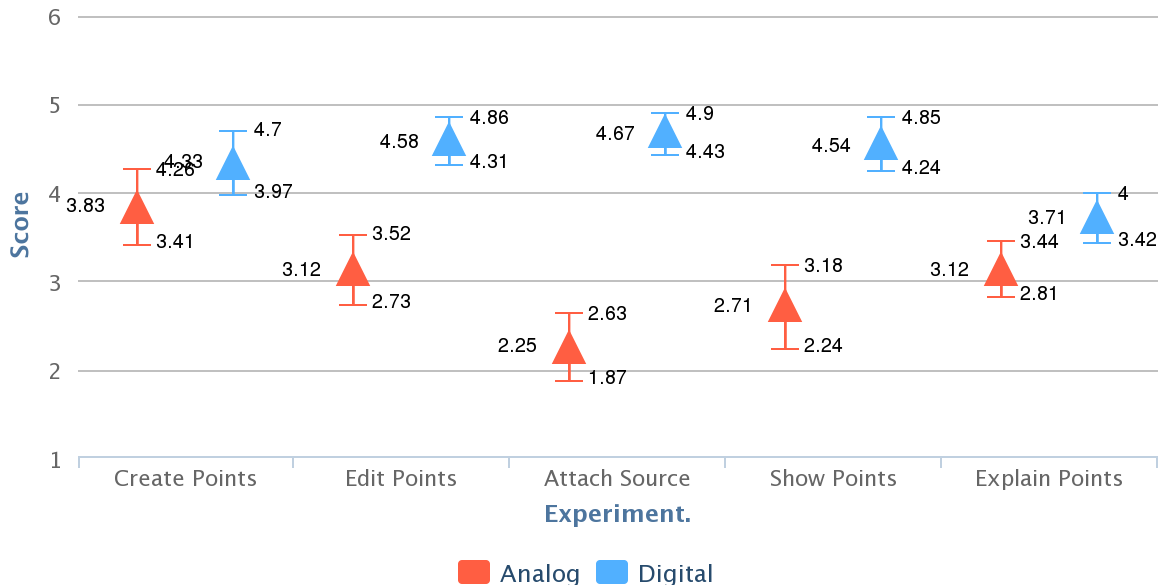
\includegraphics[width=1.0\columnwidth]{basic}
\caption{(A) Analog and Digital T.test result for usability}
\label{fig:figure1}
\end{figure}


Participants reported that it is relatively easier to conduct the tasks in the Digital environment compared to the Analog method, and that overall, the Digital environment makes creating the collaborative affinity diagram easier than the traditional method. In the Analog condition, these tasks required navigating personal space with other users, utilizing small text spaces, editing by erasing and re-writing in that small text space, and searching a large area for a target idea card. The digital condition improves on the analog environment by giving each participant their own personal space without diminishing interactivity or the opportunity for conversation. The ease of creating, editing, and attaching sources to points was deliberately engineered into our system. Editing points in the digital environment involves familiar text manipulation, while in the analog environment participants must erase and re-write information, which may discourage them from making edits. The digital environment also makes search and navigation easier, and provides multiple methods for search: via the common interactive space on the multi-touch screen, and via the list of other users' points in the private input space. We should also emphasize the impact of personal space in the digital environment; as stated above, multi-touch screens that represented common interactive space were tilted at a 30-degree angle to make conversation easier, and there was also a larger monitor that represented the common interactive space in a central location. This allowed participants to take advantage of joint eye gaze and a repository of mutual knowledge during the comment phase, while simultaneously having immediate control over the board at their fingertips. We suspect that these features contributed to participants' Ease of Use and Satisfaction with the digital system. Specifically, participants found it marginally easier to create Digital points (M= 4.17 (SD = 1.03)) compared to Analog points (M=3.17 (1.11) p \textless 0.05) and significantly easier to edit these points, attach sources, navigate between points, and create the final affinity diagram.  Participants found the Digital editing function significantly easier (M = 4.17 (1.34)) than the same process in the Analog condition (M = 2.58 (0.90), p \textless 0.01). Participants also found navigating between points in the new system (M = 4.33 (0.65)) significantly easier than in the old system (M = 2.50 (1.00), p \textless 0.01), which was one of our primary goals in designing the system. These results are aligned with participants' reports that collaborating on the affinity diagram was easier using the digital system (M = 4.00 (0.85)) than the analog system (M = 2.58(1.00), p = 0.01). Responses to these questions give us a higher level of detail about the usability of specific features. Participants' scores show us that the private input interface improves the most difficult tasks in the affinity diagram process: creating, supporting, and finding other users' points. 

\begin{figure}[!h]
\centering
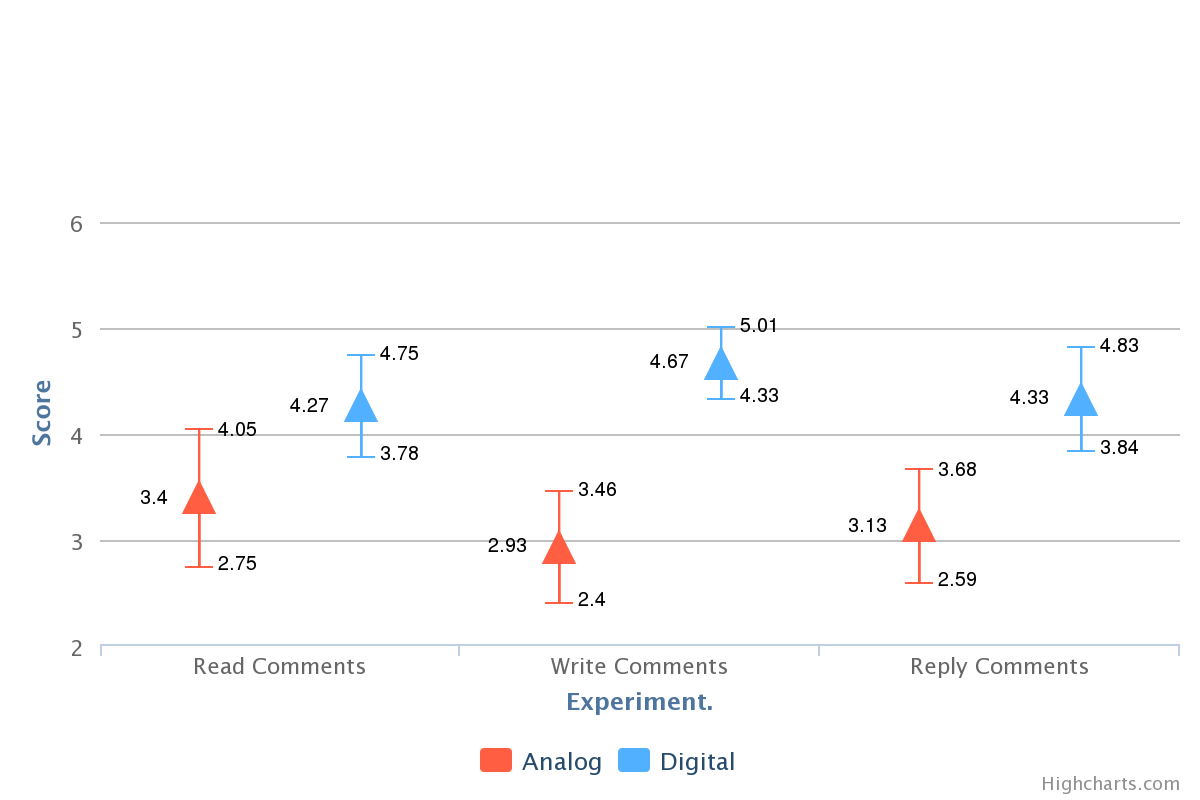
\includegraphics[width=1.0\columnwidth]{comments}
\caption{Analog and Digital T.test result for commenting}
\label{fig:figure1}
\end{figure}

These self-reports are also supported by data from users' behavior.  Figure 6 shows a clear relationship between how easily participants felt they could attach sources and show points, and how well they understood others' points. Participants felt that it was easier to attach sources in the digital system (M = 4.53 (0.67)) than in the analog system (M= 2.13 (0.85)  p \textless 0.01). This is supported by a greater number of attachments associated with each idea in the digital system (M = 5.87 (2.77)) than in the analog system (M = 2.07 (1.01), p \textless 0.01). This greater number of attachments is also associated with higher reported rates of understanding in the digital system (M = 4.07 (0.80), p = 0.04). Navigation and attachment required fewer and smaller physical movements by the participant in the digital environment. Since the environment was itself digital, it was less cumbersome to look up new sources on the Internet to support points. 

Figure 7 shows a relationship between the ease of creating the affinity diagram process and participants' satisfaction with the system as a whole. This should not be surprising, since the goal of the system was to produce a coherent, well-understood affinity diagram.

\begin{figure}[!h]
\centering
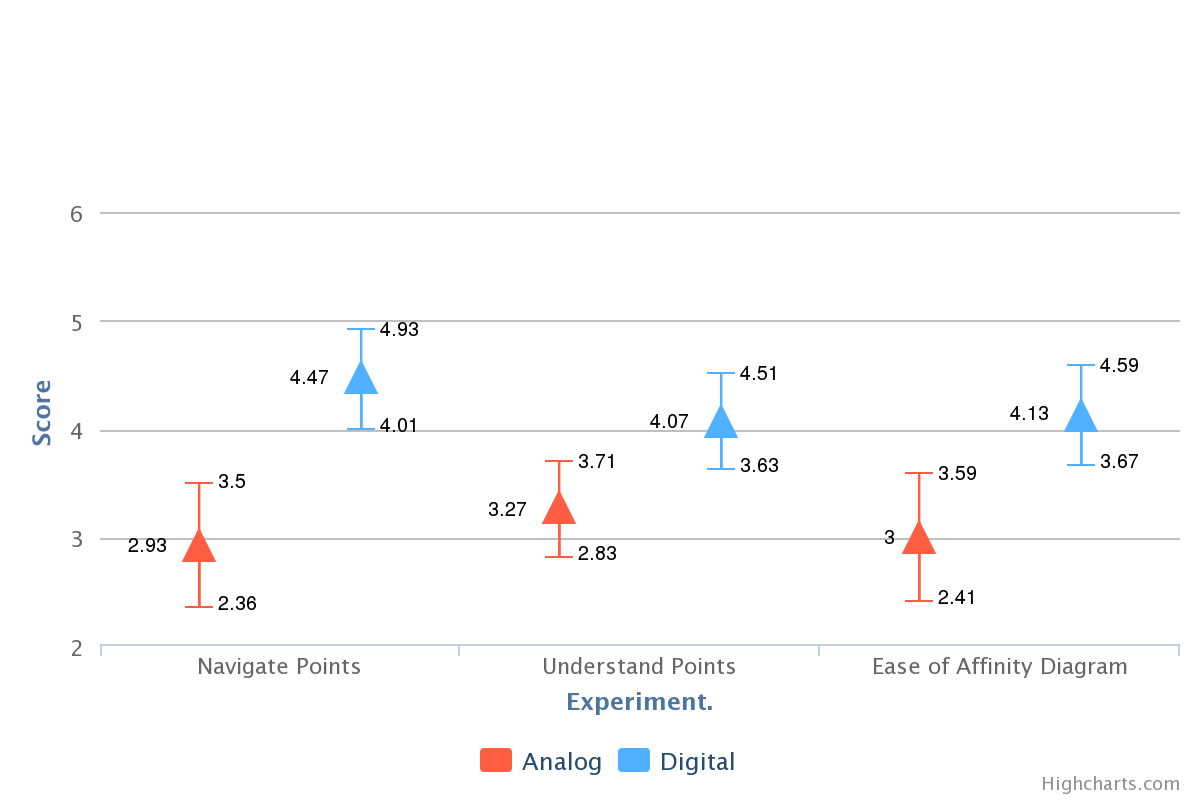
\includegraphics[width=1.0\columnwidth]{navigate}
\caption{(A) Analog and Digital T.test result for navigation}
\label{fig:figure1}
\end{figure}

The results also show that participants felt they had more flexibility in the digital environment than in the analog environment, even though the digital sessions took significantly longer. Time spent per group discussion in the Digital condition was 916.5 seconds (SD = 314.36), compared to 431.0 seconds (SD = 97.51) in the Analog condition. This may be related to different degrees of comfort: average Digital participant scored 3.92 (SD = 0.79) on this measure compared to Analog at 3.25 (SD = 1.22). Time spent in discussion also relates to the number of card manipulations and re-grouping done by participants. We coded participants' behaviors in both the Analog and Digital conditions, counting the number of times cards were moved and re-grouped, as well as the number of supporting attachments users made to their points. Card movements per participant are calculated per minute during the fourth phase of the experiment, Affinity Diagram Creation. On average, users carried out 26.75 (SD = 13.63) moves in the Digital condition compared to 6.75 (SD = 2.56) moves in the Analog condition. Since participants were more comfortable with the digital system, they may have been more inclined to extend their discussions and explore different links and re-groupings during the creation of the affinity diagram. Instead of viewing this extended time as a drawback, we view it as evidence of deeper engagement by participants with their own and others' ideas. Links and group creation demonstrate the integration of ideas into a framework for problem solving, which is the goal of affinity diagram creation. 


\begin{figure}[!h]
\centering
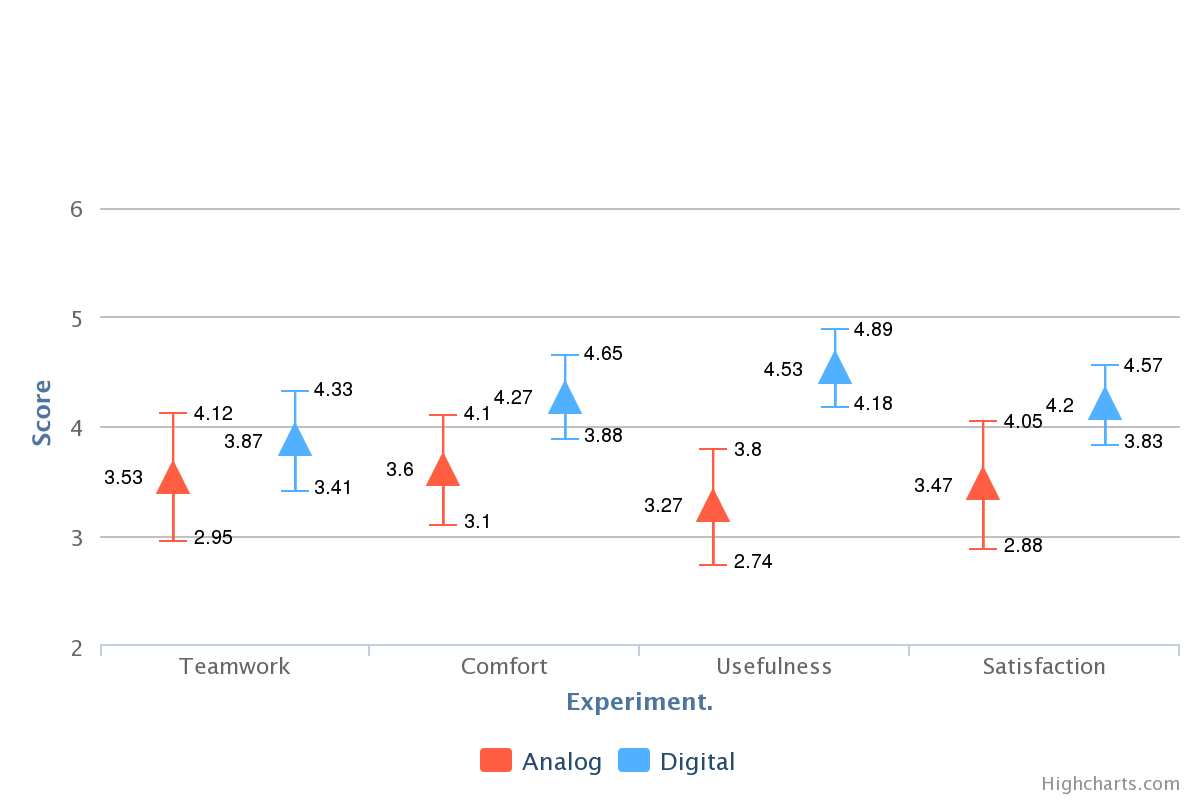
\includegraphics[width=1.0\columnwidth]{psycho}
\caption{Analog and Digital T.test result for psychometric }
\label{fig:figure1}
\end{figure}



\begin{table*}[ht]
\centering
\caption {Full Experiment Self reporting Usability Survey result }
\begin{tabular}{rrrrrrrrrrr}
  \hline
 & N & Mean & Std. Dev & Std. Err & 95\%LCI & 95\%UCI & t.test & P-Value \\ 
  \hline
  \hline
  Create Ideas AN & 15 & 3.87 & 0.92 & 0.24 & 3.36 & 4.37 & -2.32  & 0.04 \\ 
  Create Ideas DI & 15 & 4.53 & 0.92 & 0.24 & 4.03 & 5.04 &   &  \\ 
  \hline
  Edit Ideas AN & 15 & 3.27 & 1.10 & 0.28 & 2.66 & 3.88 &-5.00  & 0.00 \\ 
  Edit Ideas DI & 15 & 4.80 & 0.41 & 0.11 & 4.57 & 5.03 &   &  \\ 
    \hline
  Attach Source AN & 15 & 2.13 & 1.06 & 0.27 & 1.55 & 2.72 & -6.62   & 0.00 \\ 
  Attach Source DI & 15 & 4.53 & 0.64 & 0.17 & 4.18 & 4.89 &   &  \\ 
    \hline
  Show Ideas/Source AN & 15 & 2.87 & 1.25 & 0.32 & 2.18 & 3.56 & -3.68 & 0.00 \\ 
  Show Ideas/Source DI & 15 & 4.47 & 0.83 & 0.22 & 4.00 & 4.93 &  &  \\ 
    \hline
  Explain Ideas AN & 15 & 3.13 & 0.92 & 0.24 & 2.63 & 3.64 & -2.75  & 0.02 \\ 
  Explain Ideas DI & 15 & 3.87 & 0.83 & 0.22 & 3.40 & 4.33 &   &  \\ 
    \hline
  Navigate  AN & 15 & 2.93 & 1.03 & 0.27 & 2.36 & 3.51 & -4.07  & 0.00 \\ 
  Navigate  DI & 15 & 4.47 & 0.83 & 0.22 & 4.00 & 4.93 &   &  \\ 
    \hline
  Understand  AN & 15 & 3.27 & 0.80 & 0.21 & 2.82 & 3.71 & -3.29  & 0.01 \\ 
  Understand  DI & 15 & 4.07 & 0.80 & 0.21 & 3.62 & 4.51 &  &  \\ 
    \hline
  Read Comments AN & 15 & 3.40 & 1.18 & 0.31 & 2.74 & 4.06 & -2.30   & 0.04 \\ 
  Read Comments  DI & 15 & 4.27 & 0.88 & 0.23 & 3.78 & 4.76 &    &  \\ 
    \hline
  Write Comments AN & 15 & 2.93 & 0.96 & 0.25 & 2.40 & 3.47 & -5.77 & 0.00 \\ 
  Write Comments  DI & 15 & 4.67 & 0.62 & 0.16 & 4.32 & 5.01 &   &  \\ 
    \hline
  Reply Comments AN & 15 & 3.13 & 0.99 & 0.26 & 2.58 & 3.68 & -3.67  & 0.00 \\ 
  Reply Comments  DI & 15 & 4.33 & 0.90 & 0.23 & 3.84 & 4.83 &  &  \\ 
    \hline
  Affinity Diagram AN & 15 & 3.00 & 1.07 & 0.28 & 2.41 & 3.59 & -2.75   & 0.02 \\ 
  Affinity Diagram DI & 15 & 4.13 & 0.83 & 0.22 & 3.67 & 4.60 &  &  \\ 
  \hline
  Teamwork AN & 15 & 3.53 & 1.06 & 0.27 & 2.95 & 4.12 & -1.05   & 0.31 \\ 
  Teamwork DI & 15 & 3.87 & 0.83 & 0.22 & 3.40 & 4.33 &   &  \\ 
  \hline
  Comfort AN & 15 & 3.60 & 0.91 & 0.24 & 3.10 & 4.10 & -2.65   & 0.02 \\ 
  Comfort DI & 15 & 4.27 & 0.70 & 0.18 & 3.88 & 4.66 &  &  \\ 
  \hline
  Usefulness AN & 15 & 3.27 & 0.96 & 0.25 & 2.73 & 3.80 & -5.10 & 0.00 \\ 
  Usefulness DI & 15 & 4.53 & 0.64 & 0.17 & 4.18 & 4.89 &   &  \\ 
  \hline
  Satisfaction AN & 15 & 3.47 & 1.06 & 0.27 & 2.88 & 4.05 & -3.56   & 0.00 \\ 
  Satisfaction DI & 15 & 4.20 & 0.68 & 0.17 & 3.83 & 4.57 &    &  \\ 
   \hline
\end{tabular}
\end{table*}


\begin{table}
\centering
\caption {Performance Metrics Results}
\begin{tabular}{lrrr}
  \hline
& Analog (SD) & Digital(SD) & p-value \\ 
  \hline
  \hline
No. of source  & 2.07(1.01)  &    5.87(2.77)    &  \textless0.01    \\
no. of comments & 6.47(1.77)  &    12.87(6.16)    &  \textless0.01    \\
No. of card movement  &    7.00(3.85)& 17.0(10.82)   &  \textless0.01    \\
time AD (minutes) &    6.31(1.63)   &      9.94(3.31)      &   \textless0.01    \\ 
Speed per minute(Moves)  &    3.19(0.69)   &      5.42(2.30)      &   \textless0.05    \\ 
\hline
\end{tabular}
\end{table}


We calculated 3 objective scores for the digital system based on the industry-standard SUS instrument: Usability Score, Learn ability Score, and finally the overall SUS score. The usability score was \textbf{76.5}, which is above average, but the learn ability Score is \textbf{58.8}. Users still are not accustomed to the setup, and many said they needed more time to familiarize themselves with the system. Our system's overall score on the System Usability Scale was \textbf{72.3}, which compared to the industry standard of 68, indicates that the system is very user-friendly and should be considered a viable alternative to traditional methods. 

% Table created by stargazer v.4.5.2 by Marek Hlavac, Harvard University. E-mail: hlavac at fas.harvard.edu
% Date and time: Sat, Apr 05, 2014 - 2:09:02 AM
\begin{table}[!htbp] \centering 
  \caption{System Usability Scale Score Table} 
  \label{} 
\begin{tabular}{@{\extracolsep{5pt}}lccccc} 
\\[-1.8ex]\hline 
\hline \\[-1.8ex] 
Statistic & \multicolumn{1}{c}{N} & \multicolumn{1}{c}{Mean} & \multicolumn{1}{c}{St. Dev.}  & \multicolumn{1}{c}{Var}\\ 
\hline \\[-1.8ex] 
Usability & 15 & 76.46 & 12.49  &6.91\\ 
Learnability & 15 & 55.83 & 16.95  &9.39\\ 
SUS Score & 15 & 72.33 & 12.55  &6.95\\ 
  \hline
\normalsize 
\end{tabular} 
\end{table} 

The data we present above suggests complex relationships within and between individuals using the analog and digital systems. In order to explore several hypotheses about causal links between behavior and experience, we created linear regression models of each hypothesis. 

 Table created by stargazer v.4.5.2 by Marek Hlavac, Harvard University. E-mail: hlavac at fas.harvard.edu
 Date and time: Sat, Apr 05, 2014 - 12:54:40 AM
\begin{table}[!htbp] \centering 
 \caption{ Linear Regression on Comments} 
 \label{} 
\begin{tabular}{@{\extracolsep{6pt}}ll} 
\\[-1.8ex]\hline 
\hline \\[-1.8ex] 
 & \multicolumn{1}{c}{\textit{Number of Comments}} \\ 
\cline{2-2} 
\\[-1.8ex] &  Effect Est. (Std. Err.) \\ 
\hline \\[-1.8ex] 
 Condition & 7.363$^{***}$  (2.485) \\ 

 WComment & $-$0.108  (1.147) \\ 
  
 RComment & $-$1.785$^{**}$  (0.790) \\ 
 
 ReComment & 0.643 (0.981) \\ 
  
 Constant & 10.837$^{**}$  (4.387) \\ 
 
\hline \\[-1.8ex] 
Observations & 30 \\ 
R$^{2}$ & 0.464 \\ 
Adjusted R$^{2}$ & 0.378 \\ 
Residual Std. Error & 4.351 (df = 25) \\ 
F Statistic & 5.404$^{***}$ (df = 4; 25) \\ 
\hline 
\hline \\[-1.8ex] 
\textit{Note:}  & \multicolumn{1}{r}{$^{*}$p$<$0.1; $^{**}$p$<$0.05; $^{***}$p$<$0.01} \\ 
\normalsize 
\end{tabular} 
\end{table} 
> 

% Table created by stargazer v.4.5.2 by Marek Hlavac, Harvard University. E-mail: hlavac at fas.harvard.edu
% Date and time: Sat, Apr 05, 2014 - 12:57:48 AM
\begin{table}[!htbp] \centering 
  \caption{Linear Regression Model on Attachment} 
  \label{} 
\begin{tabular}{@{\extracolsep{5pt}}lc} 
\\[-1.8ex]\hline 
\hline \\[-1.8ex] 
 & \multicolumn{1}{c}{\textit{No of Attachment:}} \\ 
\cline{2-2} 
\\[-1.8ex] & Effect Est. (Std. Err.) \\ 
\hline \\[-1.8ex] 
 Condition & 3.784$^{***}$  (1.352) \\ 

 Attach & $-$0.393  (0.540) \\ 

 Show & 0.111  (0.423) \\ 

 explain & 1.343$^{**}$  (0.637) \\ 

 understand & $-$0.255  (0.596) \\ 

 Constant & $-$0.790  (1.812) \\ 

\hline \\[-1.8ex] 
Observations & 30 \\ 
R$^{2}$ & 0.581 \\ 
Adjusted R$^{2}$ & 0.493 \\ 
Residual Std. Error & 2.018 (df = 24) \\ 
F Statistic & 6.642$^{***}$ (df = 5; 24) \\ 
\hline 
\hline \\[-1.8ex] 
\textit{Note:}  & \multicolumn{1}{r}{$^{*}$p$<$0.1; $^{**}$p$<$0.05; $^{***}$p$<$0.01} \\ 
\normalsize 
\end{tabular} 
\end{table} 
> 
---------------
----% Table created by stargazer v.4.5.2 by Marek Hlavac, Harvard University. E-mail: hlavac at fas.harvard.edu
% Date and time: Sat, Apr 05, 2014 - 12:58:55 AM
\begin{table}[!htbp] \centering 
  \caption{Linear Regression on Move} 
  \label{} 
\begin{tabular}{@{\extracolsep{5pt}}lc} 
\\[-1.8ex]\hline 
\hline \\[-1.8ex] 
 & \multicolumn{1}{c}{\textit{No of Moves:}} \\ 
\cline{2-2} 
\\[-1.8ex] & Effect Est. (Std. Err.) \\ 
\hline \\[-1.8ex] 
 Condition & 10.005$^{***}$  (3.174) \\ 
 flexibility & $-$1.146  (1.568) \\ 
 comfort & $-$3.779$^{*}$  (1.876) \\ 
 satisfaction & 5.200$^{***}$  (1.729) \\ 
 Constant & 6.018  (7.247) \\ 
 
\hline \\[-1.8ex] 
Observations & 30 \\ 
R$^{2}$ & 0.499 \\ 
Adjusted R$^{2}$ & 0.419 \\ 
Residual Std. Error & 7.215 (df = 25) \\ 
F Statistic & 6.219$^{***}$ (df = 4; 25) \\ 
\hline 
\hline \\[-1.8ex] 
\textit{Note:}  & \multicolumn{1}{r}{$^{*}$p$<$0.1; $^{**}$p$<$0.05; $^{***}$p$<$0.01} \\ 
\normalsize 
\end{tabular} 
\end{table} 

\section{Discussion}

This experiment shows that the Digital Affinity Diagram System receives high user ratings on standard measures such as usability, learnability, and SUS, as well as more specific ratings on the mechanics of the system. Actions such as creating and navigating between ideas is easier in our system compared to the analog method. In addition, the number of sources attached to each idea is higher in the digital system, which may lead users to feel more confident about their ideas. Commenting on each other's points is also easier in the digital environment compared to analog. However, there is no significant difference between how well these systems help groups understand each other during the creation of an Affinity Diagram. Likewise, the two systems score evenly on whether they improve teamwork. The digital system can maintain the same level of teamwork despite working in an unfamiliar platform. Groups also spend more time creating the digital affinity diagram - on average, an additional 350 seconds.  While some of this time may be due to the unfamiliarity of the tool, we believe most of this time is spent making and re-forming cognitive connections within and between topics. We see evidence of enhanced engagement with ideas in the number of movements that each point undergoes in the Affinity Diagram process: 4 times more movements in our DADS system than in the analog environment. Finally, users report a higher level of satisfaction with the digital content compared to the analog content. 


\section{Conclusion}
Our system presents a clear improvement over other digital idea exchange environments, and has many advantages compared to the traditional pen-and-paper method. Based on this experiment, we can conclude that current digital methods create a more satisfying experience of organizing ideas within a team compared to traditional methods. This study shows many of the benefits our system can provide in helping users to exchange and organize their ideas better. While we have focused the current paper on the overall usability of the system and the ease of creation, enrichment, and navigation between ideas, future research may explore the innovative possibilities of the presentation feature of DADS. Focusing on presentation and comments will give us deeper insight into the group collaboration process and how it can be mediated by technology. Our system gives users the opportunity to strengthen their points and deepen their understanding of the discussion topic.  Future work may include an in-depth look at users comments, how they felt about the presentation tool, and how presentations shaped the eventual affinity diagram. We speculate that effective use of the presentation tool and comments is the main method by which users exert influence over the discussion.

This experiment also presents several avenues for future research. It is possible that exposing all participants to both methods biased them in favor of the technological method, so future experiments will make the system used a between-participants condition to increase the clarity of the research's implications. More detailed analyses could be performed on the current data to show whether there is a correlation in individual participants between ease of use and behavioral measures like number of actions taken or number of attachments made. This system also lends itself to real-world applications; if it is extended for business use, future iterations should record all idea cards and attached material in a database for re-use the next time a team within the organization discusses a similar topic. 


\section{Acknowledgments}

We would like to extend our gratitude to Tohoku University for providing laboratory facilities, Various open-source communities that supported the software development, numerous volunteers that participated in the testing phase by giving constructive feedback to improve system,  Japanese MEXT for government funding and scholarship, the team from ACM who provided the latex format and for Ubicomp 2014 for organizing the conference.

% either use a hack like flushend or balance, or manually insert
% a column break.  http://www.tex.ac.uk/cgi-bin/texfaq2html?label=balance
% multicols doesn't work because we're already in two-column mode,
% and flushend isn't awesome, so I choose balance.  See this
% for more info: http://cs.brown.edu/system/software/latex/doc/balance.pdf
%
% Note that in a perfect world balance wants to be in the first
% column of the last page.
%
% If balance doesn't work for you, you can remove that and
% hard-code a column break into the bbl file right before you
% submit:
%
% http://stackoverflow.com/questions/2149854/how-to-manually-equalize-columns-
% in-an-ieee-paper-if-using-bibtex
%
% Or, just remove \balance and give up on balancing the last page.
%
% References must be the same font size as other body text.

\bibliographystyle{acm-sigchi}
\bibliography{sample}
\end{document}
